\documentclass[1p]{elsarticle_modified}
%\bibliographystyle{elsarticle-num}

%\usepackage[colorlinks]{hyperref}
%\usepackage{abbrmath_seonhwa} %\Abb, \Ascr, \Acal ,\Abf, \Afrak
\usepackage{amsfonts}
\usepackage{amssymb}
\usepackage{amsmath}
\usepackage{amsthm}
\usepackage{scalefnt}
\usepackage{amsbsy}
\usepackage{kotex}
\usepackage{caption}
\usepackage{subfig}
\usepackage{color}
\usepackage{graphicx}
\usepackage{xcolor} %% white, black, red, green, blue, cyan, magenta, yellow
\usepackage{float}
\usepackage{setspace}
\usepackage{hyperref}

\usepackage{tikz}
\usetikzlibrary{arrows}

\usepackage{multirow}
\usepackage{array} % fixed length table
\usepackage{hhline}

%%%%%%%%%%%%%%%%%%%%%
\makeatletter
\renewcommand*\env@matrix[1][\arraystretch]{%
	\edef\arraystretch{#1}%
	\hskip -\arraycolsep
	\let\@ifnextchar\new@ifnextchar
	\array{*\c@MaxMatrixCols c}}
\makeatother %https://tex.stackexchange.com/questions/14071/how-can-i-increase-the-line-spacing-in-a-matrix
%%%%%%%%%%%%%%%

\usepackage[normalem]{ulem}

\newcommand{\msout}[1]{\ifmmode\text{\sout{\ensuremath{#1}}}\else\sout{#1}\fi}
%SOURCE: \msout is \stkout macro in https://tex.stackexchange.com/questions/20609/strikeout-in-math-mode

\newcommand{\cancel}[1]{
	\ifmmode
	{\color{red}\msout{#1}}
	\else
	{\color{red}\sout{#1}}
	\fi
}

\newcommand{\add}[1]{
	{\color{blue}\uwave{#1}}
}

\newcommand{\replace}[2]{
	\ifmmode
	{\color{red}\msout{#1}}{\color{blue}\uwave{#2}}
	\else
	{\color{red}\sout{#1}}{\color{blue}\uwave{#2}}
	\fi
}

\newcommand{\Sol}{\mathcal{S}} %segment
\newcommand{\D}{D} %diagram
\newcommand{\A}{\mathcal{A}} %arc


%%%%%%%%%%%%%%%%%%%%%%%%%%%%%5 test

\def\sl{\operatorname{\textup{SL}}(2,\Cbb)}
\def\psl{\operatorname{\textup{PSL}}(2,\Cbb)}
\def\quan{\mkern 1mu \triangleright \mkern 1mu}

\theoremstyle{definition}
\newtheorem{thm}{Theorem}[section]
\newtheorem{prop}[thm]{Proposition}
\newtheorem{lem}[thm]{Lemma}
\newtheorem{ques}[thm]{Question}
\newtheorem{cor}[thm]{Corollary}
\newtheorem{defn}[thm]{Definition}
\newtheorem{exam}[thm]{Example}
\newtheorem{rmk}[thm]{Remark}
\newtheorem{alg}[thm]{Algorithm}

\newcommand{\I}{\sqrt{-1}}
\begin{document}

%\begin{frontmatter}
%
%\title{Boundary parabolic representations of knots up to 8 crossings}
%
%%% Group authors per affiliation:
%\author{Yunhi Cho} 
%\address{Department of Mathematics, University of Seoul, Seoul, Korea}
%\ead{yhcho@uos.ac.kr}
%
%
%\author{Seonhwa Kim} %\fnref{s_kim}}
%\address{Center for Geometry and Physics, Institute for Basic Science, Pohang, 37673, Korea}
%\ead{ryeona17@ibs.re.kr}
%
%\author{Hyuk Kim}
%\address{Department of Mathematical Sciences, Seoul National University, Seoul 08826, Korea}
%\ead{hyukkim@snu.ac.kr}
%
%\author{Seokbeom Yoon}
%\address{Department of Mathematical Sciences, Seoul National University, Seoul, 08826,  Korea}
%\ead{sbyoon15@snu.ac.kr}
%
%\begin{abstract}
%We find all boundary parabolic representation of knots up to 8 crossings.
%
%\end{abstract}
%\begin{keyword}
%    \MSC[2010] 57M25 
%\end{keyword}
%
%\end{frontmatter}

%\linenumbers
%\tableofcontents
%
\newcommand\colored[1]{\textcolor{white}{\rule[-0.35ex]{0.8em}{1.4ex}}\kern-0.8em\color{red} #1}%
%\newcommand\colored[1]{\textcolor{white}{ #1}\kern-2.17ex	\textcolor{white}{ #1}\kern-1.81ex	\textcolor{white}{ #1}\kern-2.15ex\color{red}#1	}

{\Large $\underline{12a_{0852}~(K12a_{0852})}$}

\setlength{\tabcolsep}{10pt}
\renewcommand{\arraystretch}{1.6}
\vspace{1cm}\begin{tabular}{m{100pt}>{\centering\arraybackslash}m{274pt}}
\multirow{5}{120pt}{
	\centering
	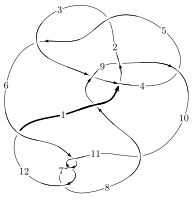
\includegraphics[width=112pt]{../../../GIT/diagram.site/Diagrams/png/1653_12a_0852.png}\\
\ \ \ A knot diagram\footnotemark}&
\allowdisplaybreaks
\textbf{Linearized knot diagam} \\
\cline{2-2}
 &
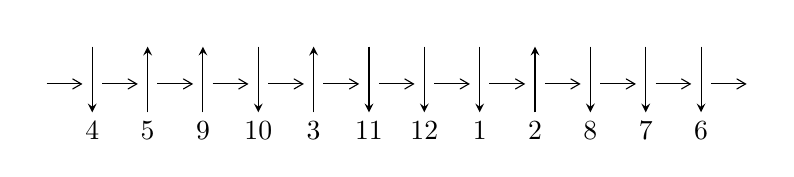
\begin{tikzpicture}[x=20pt, y=17pt]
	% nodes
	\node (C0) at (0, 0) {};
	\node (C1) at (1, 0) {};
	\node (C1U) at (1, +1) {};
	\node (C1D) at (1, -1) {4};

	\node (C2) at (2, 0) {};
	\node (C2U) at (2, +1) {};
	\node (C2D) at (2, -1) {5};

	\node (C3) at (3, 0) {};
	\node (C3U) at (3, +1) {};
	\node (C3D) at (3, -1) {9};

	\node (C4) at (4, 0) {};
	\node (C4U) at (4, +1) {};
	\node (C4D) at (4, -1) {10};

	\node (C5) at (5, 0) {};
	\node (C5U) at (5, +1) {};
	\node (C5D) at (5, -1) {3};

	\node (C6) at (6, 0) {};
	\node (C6U) at (6, +1) {};
	\node (C6D) at (6, -1) {11};

	\node (C7) at (7, 0) {};
	\node (C7U) at (7, +1) {};
	\node (C7D) at (7, -1) {12};

	\node (C8) at (8, 0) {};
	\node (C8U) at (8, +1) {};
	\node (C8D) at (8, -1) {1};

	\node (C9) at (9, 0) {};
	\node (C9U) at (9, +1) {};
	\node (C9D) at (9, -1) {2};

	\node (C10) at (10, 0) {};
	\node (C10U) at (10, +1) {};
	\node (C10D) at (10, -1) {8};

	\node (C11) at (11, 0) {};
	\node (C11U) at (11, +1) {};
	\node (C11D) at (11, -1) {7};

	\node (C12) at (12, 0) {};
	\node (C12U) at (12, +1) {};
	\node (C12D) at (12, -1) {6};
	\node (C13) at (13, 0) {};

	% arrows
	\draw[->,>={angle 60}]
	(C0) edge (C1) (C1) edge (C2) (C2) edge (C3) (C3) edge (C4) (C4) edge (C5) (C5) edge (C6) (C6) edge (C7) (C7) edge (C8) (C8) edge (C9) (C9) edge (C10) (C10) edge (C11) (C11) edge (C12) (C12) edge (C13) ;	\draw[->,>=stealth]
	(C1U) edge (C1D) (C2D) edge (C2U) (C3D) edge (C3U) (C4U) edge (C4D) (C5D) edge (C5U) (C6U) edge (C6D) (C7U) edge (C7D) (C8U) edge (C8D) (C9D) edge (C9U) (C10U) edge (C10D) (C11U) edge (C11D) (C12U) edge (C12D) ;
	\end{tikzpicture} \\
\hhline{~~} \\& 
\textbf{Solving Sequence} \\ \cline{2-2} 
 &
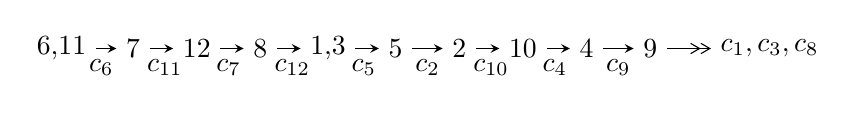
\begin{tikzpicture}[x=23pt, y=7pt]
	% node
	\node (A0) at (-1/8, 0) {6,11};
	\node (A1) at (1, 0) {7};
	\node (A2) at (2, 0) {12};
	\node (A3) at (3, 0) {8};
	\node (A4) at (65/16, 0) {1,3};
	\node (A5) at (41/8, 0) {5};
	\node (A6) at (49/8, 0) {2};
	\node (A7) at (57/8, 0) {10};
	\node (A8) at (65/8, 0) {4};
	\node (A9) at (73/8, 0) {9};
	\node (C1) at (1/2, -1) {$c_{6}$};
	\node (C2) at (3/2, -1) {$c_{11}$};
	\node (C3) at (5/2, -1) {$c_{7}$};
	\node (C4) at (7/2, -1) {$c_{12}$};
	\node (C5) at (37/8, -1) {$c_{5}$};
	\node (C6) at (45/8, -1) {$c_{2}$};
	\node (C7) at (53/8, -1) {$c_{10}$};
	\node (C8) at (61/8, -1) {$c_{4}$};
	\node (C9) at (69/8, -1) {$c_{9}$};
	\node (A10) at (11, 0) {$c_{1},c_{3},c_{8}$};

	% edge
	\draw[->,>=stealth]	
	(A0) edge (A1) (A1) edge (A2) (A2) edge (A3) (A3) edge (A4) (A4) edge (A5) (A5) edge (A6) (A6) edge (A7) (A7) edge (A8) (A8) edge (A9) ;
	\draw[->>,>={angle 60}]	
	(A9) edge (A10);
\end{tikzpicture} \\ 

\end{tabular} \\

\footnotetext{
The image of knot diagram is generated by the software ``\textbf{Draw programme}" developed by Andrew Bartholomew(\url{http://www.layer8.co.uk/maths/draw/index.htm\#Running-draw}), where we modified some parts for our purpose(\url{https://github.com/CATsTAILs/LinksPainter}).
}\phantom \\ \newline 
\centering \textbf{Ideals for irreducible components\footnotemark of $X_{\text{par}}$} 
 
\begin{align*}
I^u_{1}&=\langle 
2.17522\times10^{33} u^{103}-2.37686\times10^{33} u^{102}+\cdots+1.19004\times10^{34} b+7.34507\times10^{33},\\
\phantom{I^u_{1}}&\phantom{= \langle  }1.83944\times10^{33} u^{103}+7.61714\times10^{33} u^{102}+\cdots+1.19004\times10^{34} a+1.97168\times10^{34},\;u^{104}-2 u^{103}+\cdots+u+1\rangle \\
I^u_{2}&=\langle 
b-1,\;a,\;u-1\rangle \\
\\
\end{align*}
\raggedright * 2 irreducible components of $\dim_{\mathbb{C}}=0$, with total 105 representations.\\
\footnotetext{All coefficients of polynomials are rational numbers. But the coefficients are sometimes approximated in decimal forms when there is not enough margin.}
\newpage
\renewcommand{\arraystretch}{1}
\centering \section*{I. $I^u_{1}= \langle 2.18\times10^{33} u^{103}-2.38\times10^{33} u^{102}+\cdots+1.19\times10^{34} b+7.35\times10^{33},\;1.84\times10^{33} u^{103}+7.62\times10^{33} u^{102}+\cdots+1.19\times10^{34} a+1.97\times10^{34},\;u^{104}-2 u^{103}+\cdots+u+1 \rangle$}
\flushleft \textbf{(i) Arc colorings}\\
\begin{tabular}{m{7pt} m{180pt} m{7pt} m{180pt} }
\flushright $a_{6}=$&$\begin{pmatrix}1\\0\end{pmatrix}$ \\
\flushright $a_{11}=$&$\begin{pmatrix}0\\u\end{pmatrix}$ \\
\flushright $a_{7}=$&$\begin{pmatrix}1\\u^2\end{pmatrix}$ \\
\flushright $a_{12}=$&$\begin{pmatrix}- u\\- u^3+u\end{pmatrix}$ \\
\flushright $a_{8}=$&$\begin{pmatrix}- u^2+1\\- u^4+2 u^2\end{pmatrix}$ \\
\flushright $a_{1}=$&$\begin{pmatrix}u^3-2 u\\- u^3+u\end{pmatrix}$ \\
\flushright $a_{3}=$&$\begin{pmatrix}-0.154570 u^{103}-0.640077 u^{102}+\cdots-8.49712 u-1.65682\\-0.182786 u^{103}+0.199730 u^{102}+\cdots+1.15418 u-0.617214\end{pmatrix}$ \\
\flushright $a_{5}=$&$\begin{pmatrix}0.564505 u^{103}+0.239962 u^{102}+\cdots+6.85734 u+1.98992\\0.268856 u^{103}-0.201079 u^{102}+\cdots-1.38328 u+0.531144\end{pmatrix}$ \\
\flushright $a_{2}=$&$\begin{pmatrix}0.997344 u^{103}-1.00004 u^{102}+\cdots-3.56627 u-0.283414\\0.827859 u^{103}+0.00269680 u^{102}+\cdots-1.54179 u-0.827859\end{pmatrix}$ \\
\flushright $a_{10}=$&$\begin{pmatrix}u^5-2 u^3+u\\u^7-3 u^5+2 u^3+u\end{pmatrix}$ \\
\flushright $a_{4}=$&$\begin{pmatrix}0.560773 u^{103}+0.239997 u^{102}+\cdots+6.85749 u+1.98999\\1.30153 u^{103}-1.39251 u^{102}+\cdots-5.85230 u-1.30153\end{pmatrix}$ \\
\flushright $a_{9}=$&$\begin{pmatrix}u^{10}-5 u^8+8 u^6-3 u^4-3 u^2+1\\- u^{10}+4 u^8-5 u^6+3 u^2\end{pmatrix}$\\&\end{tabular}
\flushleft \textbf{(ii) Obstruction class $= -1$}\\~\\
\flushleft \textbf{(iii) Cusp Shapes $= -0.780657 u^{103}+6.36032 u^{102}+\cdots+24.6150 u+10.1407$}\\~\\
\newpage\renewcommand{\arraystretch}{1}
\flushleft \textbf{(iv) u-Polynomials at the component}\newline \\
\begin{tabular}{m{50pt}|m{274pt}}
Crossings & \hspace{64pt}u-Polynomials at each crossing \\
\hline $$\begin{aligned}c_{1}\end{aligned}$$&$\begin{aligned}
&u^{104}-17 u^{103}+\cdots-6 u+2
\end{aligned}$\\
\hline $$\begin{aligned}c_{2},c_{5}\end{aligned}$$&$\begin{aligned}
&u^{104}+2 u^{103}+\cdots-17 u-1
\end{aligned}$\\
\hline $$\begin{aligned}c_{3}\end{aligned}$$&$\begin{aligned}
&u^{104}+45 u^{102}+\cdots-223 u+19
\end{aligned}$\\
\hline $$\begin{aligned}c_{4}\end{aligned}$$&$\begin{aligned}
&u^{104}+2 u^{103}+\cdots+89 u+29
\end{aligned}$\\
\hline $$\begin{aligned}c_{6},c_{7},c_{11}\end{aligned}$$&$\begin{aligned}
&u^{104}+2 u^{103}+\cdots- u+1
\end{aligned}$\\
\hline $$\begin{aligned}c_{8}\end{aligned}$$&$\begin{aligned}
&u^{104}-13 u^{102}+\cdots+325815 u+31313
\end{aligned}$\\
\hline $$\begin{aligned}c_{9}\end{aligned}$$&$\begin{aligned}
&u^{104}+4 u^{103}+\cdots- u-1
\end{aligned}$\\
\hline $$\begin{aligned}c_{10},c_{12}\end{aligned}$$&$\begin{aligned}
&u^{104}-3 u^{103}+\cdots+1056 u-288
\end{aligned}$\\
\hline
\end{tabular}\\~\\
\newpage\renewcommand{\arraystretch}{1}
\flushleft \textbf{(v) Riley Polynomials at the component}\newline \\
\begin{tabular}{m{50pt}|m{274pt}}
Crossings & \hspace{64pt}Riley Polynomials at each crossing \\
\hline $$\begin{aligned}c_{1}\end{aligned}$$&$\begin{aligned}
&y^{104}-9 y^{103}+\cdots-80 y+4
\end{aligned}$\\
\hline $$\begin{aligned}c_{2},c_{5}\end{aligned}$$&$\begin{aligned}
&y^{104}-66 y^{103}+\cdots-21 y+1
\end{aligned}$\\
\hline $$\begin{aligned}c_{3}\end{aligned}$$&$\begin{aligned}
&y^{104}+90 y^{103}+\cdots-10893 y+361
\end{aligned}$\\
\hline $$\begin{aligned}c_{4}\end{aligned}$$&$\begin{aligned}
&y^{104}+106 y^{103}+\cdots+9595 y+841
\end{aligned}$\\
\hline $$\begin{aligned}c_{6},c_{7},c_{11}\end{aligned}$$&$\begin{aligned}
&y^{104}-86 y^{103}+\cdots-5 y+1
\end{aligned}$\\
\hline $$\begin{aligned}c_{8}\end{aligned}$$&$\begin{aligned}
&y^{104}-26 y^{103}+\cdots-64509499981 y+980503969
\end{aligned}$\\
\hline $$\begin{aligned}c_{9}\end{aligned}$$&$\begin{aligned}
&y^{104}-18 y^{103}+\cdots-5 y+1
\end{aligned}$\\
\hline $$\begin{aligned}c_{10},c_{12}\end{aligned}$$&$\begin{aligned}
&y^{104}+63 y^{103}+\cdots-965952 y+82944
\end{aligned}$\\
\hline
\end{tabular}\\~\\
\newpage\flushleft \textbf{(vi) Complex Volumes and Cusp Shapes}
$$\begin{array}{c|c|c}  
\text{Solutions to }I^u_{1}& \I (\text{vol} + \sqrt{-1}CS) & \text{Cusp shape}\\
 \hline 
\begin{aligned}
u &= \phantom{-}0.819897 + 0.339888 I \\
a &= -0.618092 - 0.371458 I \\
b &= \phantom{-}0.847810 + 0.105674 I\end{aligned}
 & -0.757428 + 0.259701 I & \phantom{-0.000000 } 0 \\ \hline\begin{aligned}
u &= \phantom{-}0.819897 - 0.339888 I \\
a &= -0.618092 + 0.371458 I \\
b &= \phantom{-}0.847810 - 0.105674 I\end{aligned}
 & -0.757428 - 0.259701 I & \phantom{-0.000000 } 0 \\ \hline\begin{aligned}
u &= -1.086970 + 0.359710 I \\
a &= -1.360150 - 0.080546 I \\
b &= \phantom{-}1.34875 - 0.55310 I\end{aligned}
 & \phantom{-}2.38106 - 9.69349 I & \phantom{-0.000000 } 0 \\ \hline\begin{aligned}
u &= -1.086970 - 0.359710 I \\
a &= -1.360150 + 0.080546 I \\
b &= \phantom{-}1.34875 + 0.55310 I\end{aligned}
 & \phantom{-}2.38106 + 9.69349 I & \phantom{-0.000000 } 0 \\ \hline\begin{aligned}
u &= -1.105020 + 0.306891 I \\
a &= -0.199413 - 0.213073 I \\
b &= \phantom{-}0.016100 + 1.138540 I\end{aligned}
 & -1.77784 - 3.79314 I & \phantom{-0.000000 } 0 \\ \hline\begin{aligned}
u &= -1.105020 - 0.306891 I \\
a &= -0.199413 + 0.213073 I \\
b &= \phantom{-}0.016100 - 1.138540 I\end{aligned}
 & -1.77784 + 3.79314 I & \phantom{-0.000000 } 0 \\ \hline\begin{aligned}
u &= \phantom{-}1.131960 + 0.250386 I \\
a &= -0.639350 - 0.213959 I \\
b &= \phantom{-}0.015696 - 0.221086 I\end{aligned}
 & -1.278260 - 0.518432 I & \phantom{-0.000000 } 0 \\ \hline\begin{aligned}
u &= \phantom{-}1.131960 - 0.250386 I \\
a &= -0.639350 + 0.213959 I \\
b &= \phantom{-}0.015696 + 0.221086 I\end{aligned}
 & -1.278260 + 0.518432 I & \phantom{-0.000000 } 0 \\ \hline\begin{aligned}
u &= \phantom{-}0.136123 + 0.826445 I \\
a &= -2.34710 - 0.70307 I \\
b &= \phantom{-}1.055580 - 0.268217 I\end{aligned}
 & \phantom{-}4.02249 - 5.82467 I & \phantom{-0.000000 -}0. + 9.76873 I \\ \hline\begin{aligned}
u &= \phantom{-}0.136123 - 0.826445 I \\
a &= -2.34710 + 0.70307 I \\
b &= \phantom{-}1.055580 + 0.268217 I\end{aligned}
 & \phantom{-}4.02249 + 5.82467 I & \phantom{-0.000000 } 0. - 9.76873 I\\
 \hline 
 \end{array}$$\newpage$$\begin{array}{c|c|c}  
\text{Solutions to }I^u_{1}& \I (\text{vol} + \sqrt{-1}CS) & \text{Cusp shape}\\
 \hline 
\begin{aligned}
u &= -0.012968 + 0.834781 I \\
a &= -2.87263 + 0.51707 I \\
b &= \phantom{-}1.295250 - 0.298176 I\end{aligned}
 & \phantom{-}9.32839 - 4.63448 I & \phantom{-}4.37030 + 4.68852 I \\ \hline\begin{aligned}
u &= -0.012968 - 0.834781 I \\
a &= -2.87263 - 0.51707 I \\
b &= \phantom{-}1.295250 + 0.298176 I\end{aligned}
 & \phantom{-}9.32839 + 4.63448 I & \phantom{-}4.37030 - 4.68852 I \\ \hline\begin{aligned}
u &= \phantom{-}1.107320 + 0.388542 I \\
a &= -1.317400 - 0.103258 I \\
b &= \phantom{-}1.032010 + 0.213362 I\end{aligned}
 & \phantom{-}1.05685 + 1.43205 I & \phantom{-0.000000 } 0 \\ \hline\begin{aligned}
u &= \phantom{-}1.107320 - 0.388542 I \\
a &= -1.317400 + 0.103258 I \\
b &= \phantom{-}1.032010 - 0.213362 I\end{aligned}
 & \phantom{-}1.05685 - 1.43205 I & \phantom{-0.000000 } 0 \\ \hline\begin{aligned}
u &= -0.144534 + 0.811710 I \\
a &= -2.89684 + 0.94833 I \\
b &= \phantom{-}1.35719 + 0.57614 I\end{aligned}
 & \phantom{-}5.2555 + 13.9655 I & \phantom{-0.000000 } 0. - 8.79296 I \\ \hline\begin{aligned}
u &= -0.144534 - 0.811710 I \\
a &= -2.89684 - 0.94833 I \\
b &= \phantom{-}1.35719 - 0.57614 I\end{aligned}
 & \phantom{-}5.2555 - 13.9655 I & \phantom{-0.000000 -}0. + 8.79296 I \\ \hline\begin{aligned}
u &= -1.153830 + 0.313248 I \\
a &= \phantom{-}1.274740 - 0.020552 I \\
b &= -1.36053 + 0.68227 I\end{aligned}
 & \phantom{-}2.84442 - 1.43397 I & \phantom{-0.000000 } 0 \\ \hline\begin{aligned}
u &= -1.153830 - 0.313248 I \\
a &= \phantom{-}1.274740 + 0.020552 I \\
b &= -1.36053 - 0.68227 I\end{aligned}
 & \phantom{-}2.84442 + 1.43397 I & \phantom{-0.000000 } 0 \\ \hline\begin{aligned}
u &= -0.134940 + 0.785568 I \\
a &= \phantom{-}0.90410 + 1.19582 I \\
b &= \phantom{-}0.052430 - 1.189570 I\end{aligned}
 & \phantom{-}1.14989 + 7.82651 I & -2.02077 - 8.17490 I \\ \hline\begin{aligned}
u &= -0.134940 - 0.785568 I \\
a &= \phantom{-}0.90410 - 1.19582 I \\
b &= \phantom{-}0.052430 + 1.189570 I\end{aligned}
 & \phantom{-}1.14989 - 7.82651 I & -2.02077 + 8.17490 I\\
 \hline 
 \end{array}$$\newpage$$\begin{array}{c|c|c}  
\text{Solutions to }I^u_{1}& \I (\text{vol} + \sqrt{-1}CS) & \text{Cusp shape}\\
 \hline 
\begin{aligned}
u &= \phantom{-}1.171330 + 0.286191 I \\
a &= \phantom{-}3.60617 - 1.73630 I \\
b &= -1.056690 - 0.074059 I\end{aligned}
 & \phantom{-}0.890609 - 0.882288 I & \phantom{-0.000000 } 0 \\ \hline\begin{aligned}
u &= \phantom{-}1.171330 - 0.286191 I \\
a &= \phantom{-}3.60617 + 1.73630 I \\
b &= -1.056690 + 0.074059 I\end{aligned}
 & \phantom{-}0.890609 + 0.882288 I & \phantom{-0.000000 } 0 \\ \hline\begin{aligned}
u &= -0.107809 + 0.782110 I \\
a &= \phantom{-}2.98039 - 0.66950 I \\
b &= -1.34008 - 0.74189 I\end{aligned}
 & \phantom{-}6.00776 + 5.43570 I & \phantom{-}4.84361 - 7.57014 I \\ \hline\begin{aligned}
u &= -0.107809 - 0.782110 I \\
a &= \phantom{-}2.98039 + 0.66950 I \\
b &= -1.34008 + 0.74189 I\end{aligned}
 & \phantom{-}6.00776 - 5.43570 I & \phantom{-}4.84361 + 7.57014 I \\ \hline\begin{aligned}
u &= -0.081733 + 0.774053 I \\
a &= \phantom{-}2.92878 - 1.38458 I \\
b &= -1.57005 + 0.30871 I\end{aligned}
 & \phantom{-}6.79633 + 1.59864 I & \phantom{-}6.88756 - 1.28327 I \\ \hline\begin{aligned}
u &= -0.081733 - 0.774053 I \\
a &= \phantom{-}2.92878 + 1.38458 I \\
b &= -1.57005 - 0.30871 I\end{aligned}
 & \phantom{-}6.79633 - 1.59864 I & \phantom{-}6.88756 + 1.28327 I \\ \hline\begin{aligned}
u &= \phantom{-}0.138651 + 0.759319 I \\
a &= -0.351130 - 0.209085 I \\
b &= \phantom{-}0.119000 + 0.310193 I\end{aligned}
 & \phantom{-}1.63666 - 3.24838 I & -2.97188 + 2.12306 I \\ \hline\begin{aligned}
u &= \phantom{-}0.138651 - 0.759319 I \\
a &= -0.351130 + 0.209085 I \\
b &= \phantom{-}0.119000 - 0.310193 I\end{aligned}
 & \phantom{-}1.63666 + 3.24838 I & -2.97188 - 2.12306 I \\ \hline\begin{aligned}
u &= \phantom{-}0.105697 + 0.761805 I \\
a &= \phantom{-}3.83553 + 2.76175 I \\
b &= -1.051740 + 0.109936 I\end{aligned}
 & \phantom{-}4.09016 - 2.94806 I & -10.1598 - 11.5645 I \\ \hline\begin{aligned}
u &= \phantom{-}0.105697 - 0.761805 I \\
a &= \phantom{-}3.83553 - 2.76175 I \\
b &= -1.051740 - 0.109936 I\end{aligned}
 & \phantom{-}4.09016 + 2.94806 I & -10.1598 + 11.5645 I\\
 \hline 
 \end{array}$$\newpage$$\begin{array}{c|c|c}  
\text{Solutions to }I^u_{1}& \I (\text{vol} + \sqrt{-1}CS) & \text{Cusp shape}\\
 \hline 
\begin{aligned}
u &= -1.189960 + 0.315903 I \\
a &= \phantom{-}1.89639 - 0.44180 I \\
b &= -1.53464 - 0.36870 I\end{aligned}
 & \phantom{-}3.42433 + 2.35782 I & \phantom{-0.000000 } 0 \\ \hline\begin{aligned}
u &= -1.189960 - 0.315903 I \\
a &= \phantom{-}1.89639 + 0.44180 I \\
b &= -1.53464 + 0.36870 I\end{aligned}
 & \phantom{-}3.42433 - 2.35782 I & \phantom{-0.000000 } 0 \\ \hline\begin{aligned}
u &= \phantom{-}1.218850 + 0.280045 I \\
a &= -0.58237 + 1.41538 I \\
b &= -0.570636 + 0.091864 I\end{aligned}
 & -0.11833 - 1.76625 I & \phantom{-0.000000 } 0 \\ \hline\begin{aligned}
u &= \phantom{-}1.218850 - 0.280045 I \\
a &= -0.58237 - 1.41538 I \\
b &= -0.570636 - 0.091864 I\end{aligned}
 & -0.11833 + 1.76625 I & \phantom{-0.000000 } 0 \\ \hline\begin{aligned}
u &= -0.039221 + 0.746787 I \\
a &= \phantom{-}0.167152 - 1.170260 I \\
b &= -0.567779 + 0.817936 I\end{aligned}
 & \phantom{-}3.96566 - 1.29839 I & \phantom{-}2.18497 + 4.02972 I \\ \hline\begin{aligned}
u &= -0.039221 - 0.746787 I \\
a &= \phantom{-}0.167152 + 1.170260 I \\
b &= -0.567779 - 0.817936 I\end{aligned}
 & \phantom{-}3.96566 + 1.29839 I & \phantom{-}2.18497 - 4.02972 I \\ \hline\begin{aligned}
u &= \phantom{-}0.238724 + 0.696600 I \\
a &= -1.41097 - 0.43554 I \\
b &= \phantom{-}0.893342 - 0.279263 I\end{aligned}
 & \phantom{-}1.03956 - 4.10317 I & -5.12667 + 9.90639 I \\ \hline\begin{aligned}
u &= \phantom{-}0.238724 - 0.696600 I \\
a &= -1.41097 + 0.43554 I \\
b &= \phantom{-}0.893342 + 0.279263 I\end{aligned}
 & \phantom{-}1.03956 + 4.10317 I & -5.12667 - 9.90639 I \\ \hline\begin{aligned}
u &= \phantom{-}0.082721 + 0.731305 I \\
a &= \phantom{-}0.256759 - 1.035700 I \\
b &= -0.714652 - 0.132439 I\end{aligned}
 & \phantom{-}3.33458 - 1.87793 I & \phantom{-}2.57613 + 6.72386 I \\ \hline\begin{aligned}
u &= \phantom{-}0.082721 - 0.731305 I \\
a &= \phantom{-}0.256759 + 1.035700 I \\
b &= -0.714652 + 0.132439 I\end{aligned}
 & \phantom{-}3.33458 + 1.87793 I & \phantom{-}2.57613 - 6.72386 I\\
 \hline 
 \end{array}$$\newpage$$\begin{array}{c|c|c}  
\text{Solutions to }I^u_{1}& \I (\text{vol} + \sqrt{-1}CS) & \text{Cusp shape}\\
 \hline 
\begin{aligned}
u &= -1.235630 + 0.311765 I \\
a &= \phantom{-}0.410613 - 0.014767 I \\
b &= -0.439261 - 0.886111 I\end{aligned}
 & \phantom{-}0.28138 + 5.13012 I & \phantom{-0.000000 } 0 \\ \hline\begin{aligned}
u &= -1.235630 - 0.311765 I \\
a &= \phantom{-}0.410613 + 0.014767 I \\
b &= -0.439261 + 0.886111 I\end{aligned}
 & \phantom{-}0.28138 - 5.13012 I & \phantom{-0.000000 } 0 \\ \hline\begin{aligned}
u &= -0.604637 + 0.377946 I \\
a &= -1.43689 + 1.33325 I \\
b &= \phantom{-}1.289030 + 0.537727 I\end{aligned}
 & \phantom{-}1.23076 + 9.78607 I & -3.55004 - 8.76671 I \\ \hline\begin{aligned}
u &= -0.604637 - 0.377946 I \\
a &= -1.43689 - 1.33325 I \\
b &= \phantom{-}1.289030 - 0.537727 I\end{aligned}
 & \phantom{-}1.23076 - 9.78607 I & -3.55004 + 8.76671 I \\ \hline\begin{aligned}
u &= -1.247190 + 0.379009 I \\
a &= -1.92688 + 0.79547 I \\
b &= \phantom{-}1.311450 + 0.333163 I\end{aligned}
 & \phantom{-}5.51009 + 8.99383 I & \phantom{-0.000000 } 0 \\ \hline\begin{aligned}
u &= -1.247190 - 0.379009 I \\
a &= -1.92688 - 0.79547 I \\
b &= \phantom{-}1.311450 - 0.333163 I\end{aligned}
 & \phantom{-}5.51009 - 8.99383 I & \phantom{-0.000000 } 0 \\ \hline\begin{aligned}
u &= \phantom{-}1.269870 + 0.379706 I \\
a &= -1.36939 - 1.14885 I \\
b &= \phantom{-}1.275090 + 0.263970 I\end{aligned}
 & \phantom{-}5.34644 + 0.27299 I & \phantom{-0.000000 } 0 \\ \hline\begin{aligned}
u &= \phantom{-}1.269870 - 0.379706 I \\
a &= -1.36939 + 1.14885 I \\
b &= \phantom{-}1.275090 - 0.263970 I\end{aligned}
 & \phantom{-}5.34644 - 0.27299 I & \phantom{-0.000000 } 0 \\ \hline\begin{aligned}
u &= \phantom{-}1.32911\phantom{ +0.000000I} \\
a &= -0.752093\phantom{ +0.000000I} \\
b &= -1.50687\phantom{ +0.000000I}\end{aligned}
 & -1.93259\phantom{ +0.000000I} & \phantom{-0.000000 } 0 \\ \hline\begin{aligned}
u &= -0.294200 + 0.595315 I \\
a &= -1.26888 + 0.93132 I \\
b &= \phantom{-}1.237090 - 0.501458 I\end{aligned}
 & \phantom{-}2.26017 - 6.27429 I & -1.37179 + 2.81174 I\\
 \hline 
 \end{array}$$\newpage$$\begin{array}{c|c|c}  
\text{Solutions to }I^u_{1}& \I (\text{vol} + \sqrt{-1}CS) & \text{Cusp shape}\\
 \hline 
\begin{aligned}
u &= -0.294200 - 0.595315 I \\
a &= -1.26888 - 0.93132 I \\
b &= \phantom{-}1.237090 + 0.501458 I\end{aligned}
 & \phantom{-}2.26017 + 6.27429 I & -1.37179 - 2.81174 I \\ \hline\begin{aligned}
u &= \phantom{-}0.497394 + 0.439590 I \\
a &= -1.36564 - 0.72878 I \\
b &= \phantom{-}0.802243 - 0.161085 I\end{aligned}
 & -0.66419 - 1.68719 I & -11.39599 + 8.12073 I \\ \hline\begin{aligned}
u &= \phantom{-}0.497394 - 0.439590 I \\
a &= -1.36564 + 0.72878 I \\
b &= \phantom{-}0.802243 + 0.161085 I\end{aligned}
 & -0.66419 + 1.68719 I & -11.39599 - 8.12073 I \\ \hline\begin{aligned}
u &= \phantom{-}1.301770 + 0.309962 I \\
a &= -1.097610 + 0.496242 I \\
b &= -0.710921 - 0.827783 I\end{aligned}
 & -0.22651 - 2.50873 I & \phantom{-0.000000 } 0 \\ \hline\begin{aligned}
u &= \phantom{-}1.301770 - 0.309962 I \\
a &= -1.097610 - 0.496242 I \\
b &= -0.710921 + 0.827783 I\end{aligned}
 & -0.22651 + 2.50873 I & \phantom{-0.000000 } 0 \\ \hline\begin{aligned}
u &= -1.320810 + 0.229375 I \\
a &= -0.168377 - 0.148303 I \\
b &= \phantom{-}0.496393 - 0.597888 I\end{aligned}
 & -4.96158 + 3.74028 I & \phantom{-0.000000 } 0 \\ \hline\begin{aligned}
u &= -1.320810 - 0.229375 I \\
a &= -0.168377 + 0.148303 I \\
b &= \phantom{-}0.496393 + 0.597888 I\end{aligned}
 & -4.96158 - 3.74028 I & \phantom{-0.000000 } 0 \\ \hline\begin{aligned}
u &= \phantom{-}1.357340 + 0.036829 I \\
a &= -0.64481 + 1.79711 I \\
b &= -1.121420 + 0.753763 I\end{aligned}
 & -3.40531 - 3.28760 I & \phantom{-0.000000 } 0 \\ \hline\begin{aligned}
u &= \phantom{-}1.357340 - 0.036829 I \\
a &= -0.64481 - 1.79711 I \\
b &= -1.121420 - 0.753763 I\end{aligned}
 & -3.40531 + 3.28760 I & \phantom{-0.000000 } 0 \\ \hline\begin{aligned}
u &= -0.586602 + 0.257849 I \\
a &= \phantom{-}0.522102 - 0.255402 I \\
b &= \phantom{-}0.106387 - 1.029130 I\end{aligned}
 & -2.46224 + 4.23705 I & -7.70872 - 7.47519 I\\
 \hline 
 \end{array}$$\newpage$$\begin{array}{c|c|c}  
\text{Solutions to }I^u_{1}& \I (\text{vol} + \sqrt{-1}CS) & \text{Cusp shape}\\
 \hline 
\begin{aligned}
u &= -0.586602 - 0.257849 I \\
a &= \phantom{-}0.522102 + 0.255402 I \\
b &= \phantom{-}0.106387 + 1.029130 I\end{aligned}
 & -2.46224 - 4.23705 I & -7.70872 + 7.47519 I \\ \hline\begin{aligned}
u &= -1.323900 + 0.311663 I \\
a &= -0.497700 + 0.855032 I \\
b &= -0.766085 + 0.188074 I\end{aligned}
 & -1.09041 + 5.66082 I & \phantom{-0.000000 } 0 \\ \hline\begin{aligned}
u &= -1.323900 - 0.311663 I \\
a &= -0.497700 - 0.855032 I \\
b &= -0.766085 - 0.188074 I\end{aligned}
 & -1.09041 - 5.66082 I & \phantom{-0.000000 } 0 \\ \hline\begin{aligned}
u &= \phantom{-}1.320340 + 0.332094 I \\
a &= \phantom{-}0.84342 + 1.93940 I \\
b &= -1.60232 - 0.26907 I\end{aligned}
 & \phantom{-}2.39939 - 5.59260 I & \phantom{-0.000000 } 0 \\ \hline\begin{aligned}
u &= \phantom{-}1.320340 - 0.332094 I \\
a &= \phantom{-}0.84342 - 1.93940 I \\
b &= -1.60232 + 0.26907 I\end{aligned}
 & \phantom{-}2.39939 + 5.59260 I & \phantom{-0.000000 } 0 \\ \hline\begin{aligned}
u &= -1.364830 + 0.013621 I \\
a &= -0.14110 - 2.80359 I \\
b &= -0.944317 - 0.153085 I\end{aligned}
 & -4.84420 + 0.57804 I & \phantom{-0.000000 } 0 \\ \hline\begin{aligned}
u &= -1.364830 - 0.013621 I \\
a &= -0.14110 + 2.80359 I \\
b &= -0.944317 + 0.153085 I\end{aligned}
 & -4.84420 - 0.57804 I & \phantom{-0.000000 } 0 \\ \hline\begin{aligned}
u &= \phantom{-}1.340460 + 0.271297 I \\
a &= -1.19962 - 1.01951 I \\
b &= \phantom{-}0.322997 - 0.951799 I\end{aligned}
 & -5.64992 - 2.03615 I & \phantom{-0.000000 } 0 \\ \hline\begin{aligned}
u &= \phantom{-}1.340460 - 0.271297 I \\
a &= -1.19962 + 1.01951 I \\
b &= \phantom{-}0.322997 + 0.951799 I\end{aligned}
 & -5.64992 + 2.03615 I & \phantom{-0.000000 } 0 \\ \hline\begin{aligned}
u &= -0.158685 + 0.610936 I \\
a &= -1.300790 - 0.327447 I \\
b &= \phantom{-}0.228459 + 0.869260 I\end{aligned}
 & -0.96137 - 1.25908 I & -4.98451 + 0.66680 I\\
 \hline 
 \end{array}$$\newpage$$\begin{array}{c|c|c}  
\text{Solutions to }I^u_{1}& \I (\text{vol} + \sqrt{-1}CS) & \text{Cusp shape}\\
 \hline 
\begin{aligned}
u &= -0.158685 - 0.610936 I \\
a &= -1.300790 + 0.327447 I \\
b &= \phantom{-}0.228459 - 0.869260 I\end{aligned}
 & -0.96137 + 1.25908 I & -4.98451 - 0.66680 I \\ \hline\begin{aligned}
u &= -1.333430 + 0.326258 I \\
a &= \phantom{-}2.27280 - 3.29785 I \\
b &= -1.051820 - 0.133392 I\end{aligned}
 & -0.43475 + 6.88567 I & \phantom{-0.000000 } 0 \\ \hline\begin{aligned}
u &= -1.333430 - 0.326258 I \\
a &= \phantom{-}2.27280 + 3.29785 I \\
b &= -1.051820 + 0.133392 I\end{aligned}
 & -0.43475 - 6.88567 I & \phantom{-0.000000 } 0 \\ \hline\begin{aligned}
u &= \phantom{-}1.334910 + 0.336617 I \\
a &= \phantom{-}1.73924 + 2.18490 I \\
b &= -1.32785 + 0.78054 I\end{aligned}
 & \phantom{-}1.47378 - 9.47675 I & \phantom{-0.000000 } 0 \\ \hline\begin{aligned}
u &= \phantom{-}1.334910 - 0.336617 I \\
a &= \phantom{-}1.73924 - 2.18490 I \\
b &= -1.32785 - 0.78054 I\end{aligned}
 & \phantom{-}1.47378 + 9.47675 I & \phantom{-0.000000 } 0 \\ \hline\begin{aligned}
u &= \phantom{-}0.621098\phantom{ +0.000000I} \\
a &= -0.599919\phantom{ +0.000000I} \\
b &= \phantom{-}0.141868\phantom{ +0.000000I}\end{aligned}
 & -1.24720\phantom{ +0.000000I} & -8.65320\phantom{ +0.000000I} \\ \hline\begin{aligned}
u &= \phantom{-}1.365160 + 0.233330 I \\
a &= \phantom{-}0.375504 - 0.313013 I \\
b &= \phantom{-}1.183030 + 0.536242 I\end{aligned}
 & -2.91793 + 3.29629 I & \phantom{-0.000000 } 0 \\ \hline\begin{aligned}
u &= \phantom{-}1.365160 - 0.233330 I \\
a &= \phantom{-}0.375504 + 0.313013 I \\
b &= \phantom{-}1.183030 - 0.536242 I\end{aligned}
 & -2.91793 - 3.29629 I & \phantom{-0.000000 } 0 \\ \hline\begin{aligned}
u &= -1.350210 + 0.324204 I \\
a &= \phantom{-}0.0340088 - 0.0616224 I \\
b &= \phantom{-}0.161165 - 0.365219 I\end{aligned}
 & -3.05646 + 7.17585 I & \phantom{-0.000000 } 0 \\ \hline\begin{aligned}
u &= -1.350210 - 0.324204 I \\
a &= \phantom{-}0.0340088 + 0.0616224 I \\
b &= \phantom{-}0.161165 + 0.365219 I\end{aligned}
 & -3.05646 - 7.17585 I & \phantom{-0.000000 } 0\\
 \hline 
 \end{array}$$\newpage$$\begin{array}{c|c|c}  
\text{Solutions to }I^u_{1}& \I (\text{vol} + \sqrt{-1}CS) & \text{Cusp shape}\\
 \hline 
\begin{aligned}
u &= \phantom{-}1.349480 + 0.336718 I \\
a &= \phantom{-}1.50306 + 0.13604 I \\
b &= \phantom{-}0.076257 + 1.214800 I\end{aligned}
 & -3.52490 - 11.88240 I & \phantom{-0.000000 } 0 \\ \hline\begin{aligned}
u &= \phantom{-}1.349480 - 0.336718 I \\
a &= \phantom{-}1.50306 - 0.13604 I \\
b &= \phantom{-}0.076257 - 1.214800 I\end{aligned}
 & -3.52490 + 11.88240 I & \phantom{-0.000000 } 0 \\ \hline\begin{aligned}
u &= \phantom{-}1.392200 + 0.040896 I \\
a &= \phantom{-}0.41176 + 1.35567 I \\
b &= \phantom{-}0.189123 + 1.116580 I\end{aligned}
 & -8.55437 - 5.02075 I & \phantom{-0.000000 } 0 \\ \hline\begin{aligned}
u &= \phantom{-}1.392200 - 0.040896 I \\
a &= \phantom{-}0.41176 - 1.35567 I \\
b &= \phantom{-}0.189123 - 1.116580 I\end{aligned}
 & -8.55437 + 5.02075 I & \phantom{-0.000000 } 0 \\ \hline\begin{aligned}
u &= -1.393450 + 0.083248 I \\
a &= -0.382891 + 0.981947 I \\
b &= \phantom{-}0.847847 + 0.366478 I\end{aligned}
 & -6.65127 + 3.23336 I & \phantom{-0.000000 } 0 \\ \hline\begin{aligned}
u &= -1.393450 - 0.083248 I \\
a &= -0.382891 - 0.981947 I \\
b &= \phantom{-}0.847847 - 0.366478 I\end{aligned}
 & -6.65127 - 3.23336 I & \phantom{-0.000000 } 0 \\ \hline\begin{aligned}
u &= -1.371250 + 0.280465 I \\
a &= -0.453878 + 1.001390 I \\
b &= \phantom{-}0.850252 + 0.379510 I\end{aligned}
 & -4.02838 + 7.63331 I & \phantom{-0.000000 } 0 \\ \hline\begin{aligned}
u &= -1.371250 - 0.280465 I \\
a &= -0.453878 - 1.001390 I \\
b &= \phantom{-}0.850252 - 0.379510 I\end{aligned}
 & -4.02838 - 7.63331 I & \phantom{-0.000000 } 0 \\ \hline\begin{aligned}
u &= -1.354630 + 0.357246 I \\
a &= -1.37123 + 1.50720 I \\
b &= \phantom{-}1.063730 + 0.305774 I\end{aligned}
 & -0.67161 + 10.08760 I & \phantom{-0.000000 } 0 \\ \hline\begin{aligned}
u &= -1.354630 - 0.357246 I \\
a &= -1.37123 - 1.50720 I \\
b &= \phantom{-}1.063730 - 0.305774 I\end{aligned}
 & -0.67161 - 10.08760 I & \phantom{-0.000000 } 0\\
 \hline 
 \end{array}$$\newpage$$\begin{array}{c|c|c}  
\text{Solutions to }I^u_{1}& \I (\text{vol} + \sqrt{-1}CS) & \text{Cusp shape}\\
 \hline 
\begin{aligned}
u &= \phantom{-}1.357480 + 0.349121 I \\
a &= -1.64850 - 2.17322 I \\
b &= \phantom{-}1.35890 - 0.59148 I\end{aligned}
 & \phantom{-}0.5224 - 18.1526 I & \phantom{-0.000000 } 0 \\ \hline\begin{aligned}
u &= \phantom{-}1.357480 - 0.349121 I \\
a &= -1.64850 + 2.17322 I \\
b &= \phantom{-}1.35890 + 0.59148 I\end{aligned}
 & \phantom{-}0.5224 + 18.1526 I & \phantom{-0.000000 } 0 \\ \hline\begin{aligned}
u &= -1.408100 + 0.014929 I \\
a &= \phantom{-}0.117428 - 0.268962 I \\
b &= \phantom{-}0.493413 - 0.253339 I\end{aligned}
 & -7.53758 + 0.06657 I & \phantom{-0.000000 } 0 \\ \hline\begin{aligned}
u &= -1.408100 - 0.014929 I \\
a &= \phantom{-}0.117428 + 0.268962 I \\
b &= \phantom{-}0.493413 + 0.253339 I\end{aligned}
 & -7.53758 - 0.06657 I & \phantom{-0.000000 } 0 \\ \hline\begin{aligned}
u &= \phantom{-}1.409240 + 0.065039 I \\
a &= \phantom{-}0.12694 - 1.58323 I \\
b &= \phantom{-}1.28505 - 0.59078 I\end{aligned}
 & -5.09313 - 11.01120 I & \phantom{-0.000000 } 0 \\ \hline\begin{aligned}
u &= \phantom{-}1.409240 - 0.065039 I \\
a &= \phantom{-}0.12694 + 1.58323 I \\
b &= \phantom{-}1.28505 + 0.59078 I\end{aligned}
 & -5.09313 + 11.01120 I & \phantom{-0.000000 } 0 \\ \hline\begin{aligned}
u &= -0.435976 + 0.239765 I \\
a &= \phantom{-}0.86661 - 1.89922 I \\
b &= -1.191680 - 0.582430 I\end{aligned}
 & \phantom{-}2.08857 + 2.52807 I & -0.32506 - 8.71630 I \\ \hline\begin{aligned}
u &= -0.435976 - 0.239765 I \\
a &= \phantom{-}0.86661 + 1.89922 I \\
b &= -1.191680 + 0.582430 I\end{aligned}
 & \phantom{-}2.08857 - 2.52807 I & -0.32506 + 8.71630 I \\ \hline\begin{aligned}
u &= \phantom{-}0.449559 + 0.091341 I \\
a &= \phantom{-}0.46059 + 4.92050 I \\
b &= -0.953699 + 0.055151 I\end{aligned}
 & \phantom{-}0.728992 - 0.299030 I & \phantom{-}7.0296 - 19.8342 I \\ \hline\begin{aligned}
u &= \phantom{-}0.449559 - 0.091341 I \\
a &= \phantom{-}0.46059 - 4.92050 I \\
b &= -0.953699 - 0.055151 I\end{aligned}
 & \phantom{-}0.728992 + 0.299030 I & \phantom{-}7.0296 + 19.8342 I\\
 \hline 
 \end{array}$$\newpage$$\begin{array}{c|c|c}  
\text{Solutions to }I^u_{1}& \I (\text{vol} + \sqrt{-1}CS) & \text{Cusp shape}\\
 \hline 
\begin{aligned}
u &= \phantom{-}0.198188 + 0.402789 I \\
a &= -0.984161 - 0.454357 I \\
b &= \phantom{-}0.189920 + 0.365207 I\end{aligned}
 & -0.424686 - 1.170030 I & -5.91811 + 4.92395 I \\ \hline\begin{aligned}
u &= \phantom{-}0.198188 - 0.402789 I \\
a &= -0.984161 + 0.454357 I \\
b &= \phantom{-}0.189920 - 0.365207 I\end{aligned}
 & -0.424686 + 1.170030 I & -5.91811 - 4.92395 I \\ \hline\begin{aligned}
u &= -0.229242 + 0.271377 I \\
a &= \phantom{-}0.49573 - 1.39916 I \\
b &= -1.242340 + 0.280456 I\end{aligned}
 & \phantom{-}2.66352 - 0.40407 I & \phantom{-}2.91521 - 3.41969 I \\ \hline\begin{aligned}
u &= -0.229242 - 0.271377 I \\
a &= \phantom{-}0.49573 + 1.39916 I \\
b &= -1.242340 - 0.280456 I\end{aligned}
 & \phantom{-}2.66352 + 0.40407 I & \phantom{-}2.91521 + 3.41969 I\\
 \hline 
 \end{array}$$\newpage\newpage\renewcommand{\arraystretch}{1}
\centering \section*{II. $I^u_{2}= \langle b-1,\;a,\;u-1 \rangle$}
\flushleft \textbf{(i) Arc colorings}\\
\begin{tabular}{m{7pt} m{180pt} m{7pt} m{180pt} }
\flushright $a_{6}=$&$\begin{pmatrix}1\\0\end{pmatrix}$ \\
\flushright $a_{11}=$&$\begin{pmatrix}0\\1\end{pmatrix}$ \\
\flushright $a_{7}=$&$\begin{pmatrix}1\\1\end{pmatrix}$ \\
\flushright $a_{12}=$&$\begin{pmatrix}-1\\0\end{pmatrix}$ \\
\flushright $a_{8}=$&$\begin{pmatrix}0\\1\end{pmatrix}$ \\
\flushright $a_{1}=$&$\begin{pmatrix}-1\\0\end{pmatrix}$ \\
\flushright $a_{3}=$&$\begin{pmatrix}0\\1\end{pmatrix}$ \\
\flushright $a_{5}=$&$\begin{pmatrix}1\\1\end{pmatrix}$ \\
\flushright $a_{2}=$&$\begin{pmatrix}-1\\0\end{pmatrix}$ \\
\flushright $a_{10}=$&$\begin{pmatrix}0\\1\end{pmatrix}$ \\
\flushright $a_{4}=$&$\begin{pmatrix}1\\0\end{pmatrix}$ \\
\flushright $a_{9}=$&$\begin{pmatrix}-1\\1\end{pmatrix}$\\&\end{tabular}
\flushleft \textbf{(ii) Obstruction class $= 1$}\\~\\
\flushleft \textbf{(iii) Cusp Shapes $= 0$}\\~\\
\newpage\renewcommand{\arraystretch}{1}
\flushleft \textbf{(iv) u-Polynomials at the component}\newline \\
\begin{tabular}{m{50pt}|m{274pt}}
Crossings & \hspace{64pt}u-Polynomials at each crossing \\
\hline $$\begin{aligned}c_{1},c_{10},c_{12}\end{aligned}$$&$\begin{aligned}
&u
\end{aligned}$\\
\hline $$\begin{aligned}c_{2},c_{11}\end{aligned}$$&$\begin{aligned}
&u+1
\end{aligned}$\\
\hline $$\begin{aligned}c_{3},c_{4},c_{5}\\c_{6},c_{7},c_{8}\\c_{9}\end{aligned}$$&$\begin{aligned}
&u-1
\end{aligned}$\\
\hline
\end{tabular}\\~\\
\newpage\renewcommand{\arraystretch}{1}
\flushleft \textbf{(v) Riley Polynomials at the component}\newline \\
\begin{tabular}{m{50pt}|m{274pt}}
Crossings & \hspace{64pt}Riley Polynomials at each crossing \\
\hline $$\begin{aligned}c_{1},c_{10},c_{12}\end{aligned}$$&$\begin{aligned}
&y
\end{aligned}$\\
\hline $$\begin{aligned}c_{2},c_{3},c_{4}\\c_{5},c_{6},c_{7}\\c_{8},c_{9},c_{11}\end{aligned}$$&$\begin{aligned}
&y-1
\end{aligned}$\\
\hline
\end{tabular}\\~\\
\newpage\flushleft \textbf{(vi) Complex Volumes and Cusp Shapes}
$$\begin{array}{c|c|c}  
\text{Solutions to }I^u_{2}& \I (\text{vol} + \sqrt{-1}CS) & \text{Cusp shape}\\
 \hline 
\begin{aligned}
u &= \phantom{-}1.00000\phantom{ +0.000000I} \\
a &= \phantom{-0.000000 } 0 \\
b &= \phantom{-}1.00000\phantom{ +0.000000I}\end{aligned}
 & \phantom{-0.000000 } 0 & \phantom{-0.000000 } 0\\
 \hline 
 \end{array}$$\newpage
\newpage\renewcommand{\arraystretch}{1}
\centering \section*{ III. u-Polynomials}
\begin{tabular}{m{50pt}|m{274pt}}
Crossings & \hspace{64pt}u-Polynomials at each crossing \\
\hline $$\begin{aligned}c_{1}\end{aligned}$$&$\begin{aligned}
&u(u^{104}-17 u^{103}+\cdots-6 u+2)
\end{aligned}$\\
\hline $$\begin{aligned}c_{2}\end{aligned}$$&$\begin{aligned}
&(u+1)(u^{104}+2 u^{103}+\cdots-17 u-1)
\end{aligned}$\\
\hline $$\begin{aligned}c_{3}\end{aligned}$$&$\begin{aligned}
&(u-1)(u^{104}+45 u^{102}+\cdots-223 u+19)
\end{aligned}$\\
\hline $$\begin{aligned}c_{4}\end{aligned}$$&$\begin{aligned}
&(u-1)(u^{104}+2 u^{103}+\cdots+89 u+29)
\end{aligned}$\\
\hline $$\begin{aligned}c_{5}\end{aligned}$$&$\begin{aligned}
&(u-1)(u^{104}+2 u^{103}+\cdots-17 u-1)
\end{aligned}$\\
\hline $$\begin{aligned}c_{6},c_{7}\end{aligned}$$&$\begin{aligned}
&(u-1)(u^{104}+2 u^{103}+\cdots- u+1)
\end{aligned}$\\
\hline $$\begin{aligned}c_{8}\end{aligned}$$&$\begin{aligned}
&(u-1)(u^{104}-13 u^{102}+\cdots+325815 u+31313)
\end{aligned}$\\
\hline $$\begin{aligned}c_{9}\end{aligned}$$&$\begin{aligned}
&(u-1)(u^{104}+4 u^{103}+\cdots- u-1)
\end{aligned}$\\
\hline $$\begin{aligned}c_{10},c_{12}\end{aligned}$$&$\begin{aligned}
&u(u^{104}-3 u^{103}+\cdots+1056 u-288)
\end{aligned}$\\
\hline $$\begin{aligned}c_{11}\end{aligned}$$&$\begin{aligned}
&(u+1)(u^{104}+2 u^{103}+\cdots- u+1)
\end{aligned}$\\
\hline
\end{tabular}\newpage\renewcommand{\arraystretch}{1}
\centering \section*{ IV. Riley Polynomials}
\begin{tabular}{m{50pt}|m{274pt}}
Crossings & \hspace{64pt}Riley Polynomials at each crossing \\
\hline $$\begin{aligned}c_{1}\end{aligned}$$&$\begin{aligned}
&y(y^{104}-9 y^{103}+\cdots-80 y+4)
\end{aligned}$\\
\hline $$\begin{aligned}c_{2},c_{5}\end{aligned}$$&$\begin{aligned}
&(y-1)(y^{104}-66 y^{103}+\cdots-21 y+1)
\end{aligned}$\\
\hline $$\begin{aligned}c_{3}\end{aligned}$$&$\begin{aligned}
&(y-1)(y^{104}+90 y^{103}+\cdots-10893 y+361)
\end{aligned}$\\
\hline $$\begin{aligned}c_{4}\end{aligned}$$&$\begin{aligned}
&(y-1)(y^{104}+106 y^{103}+\cdots+9595 y+841)
\end{aligned}$\\
\hline $$\begin{aligned}c_{6},c_{7},c_{11}\end{aligned}$$&$\begin{aligned}
&(y-1)(y^{104}-86 y^{103}+\cdots-5 y+1)
\end{aligned}$\\
\hline $$\begin{aligned}c_{8}\end{aligned}$$&$\begin{aligned}
&(y-1)(y^{104}-26 y^{103}+\cdots-6.45095\times10^{10} y+9.80504\times10^{8})
\end{aligned}$\\
\hline $$\begin{aligned}c_{9}\end{aligned}$$&$\begin{aligned}
&(y-1)(y^{104}-18 y^{103}+\cdots-5 y+1)
\end{aligned}$\\
\hline $$\begin{aligned}c_{10},c_{12}\end{aligned}$$&$\begin{aligned}
&y(y^{104}+63 y^{103}+\cdots-965952 y+82944)
\end{aligned}$\\
\hline
\end{tabular}
\vskip 2pc
\end{document}